\scanpage{131}
Résulte par récurrence \deleted{\unsure{sur}} du

\margin{\figure{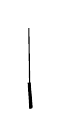
\begin{tikzpicture}[x=0.3cm,y=0.3cm]\draw (0,3.4)--(0.05,0);\draw[line width=1pt] (0.01,1.1)--(0.08,0);\draw (0.05,1.1)--(0.14,0.04);\end{tikzpicture}}}
\uline{Lemme}. $X$ \deleted{séparable}\inserted{\deleted{\unsure{réduit}}\unsure{séparable}} propre sur le corps $k$, et \deleted{soit} $X_1$ et $X_2$ deux parties fermées de $X$, séparables sur $k$, telles que $X=\cup X_1\cup X_2$. Alors $\underline{\operatorname{Pic}}_{X/k}\text{---}\underline{\operatorname{Pic}}_{X_1/k}\times\underline{\operatorname{Pic}}_{X_2/k}$ est représentable par morphismes affines.

\inserted{\deleted{Si $X_1\cap X_2=\varnothing$, \unsure{on a} \unsure{donc}} Supposons $X_1\cap X_2\ne\varnothing$}
Comme les faisceaux en jeu sont compatibles \deleted{\unsure{pour}} aux changements fid plats quasi cpcts, et que \deleted{les} morphismes de cette nature sont des morphismes de descente effective pour les morphismes affines, rien n'est changé en faisant un changement de base $\unsure{\bar k'|k'}/k$, où $k'/k$ est une extension de corps. On peut donc se ramener au cas où $F=X_1\cap X_2$ a un pt rat. sur $k$, i.e. une section $g$ sur $S=\operatorname{Spec}k$), On applique alors le th. avec $X'=X_1\amalg X_2$.

\deleted{\unsure{Dém.}}

\uline{Attention}. Commençons par le corollaire: se ramener au cas où $k$ est alg. clos, et $X$ connexe, ce qui nous ramène dans le \uline{lemme} dans le cas où $X_1$ et $X_2$ sont \uline{connexes} et $X_1\cap X_2$ a un pt rat. /$k$. \unsure{On est ds les conditions du}

\margin{\diagram{\begin{tikzcd}[column sep=small,row sep=large]
\underline{\operatorname{Pic}}_X\arrow[r,"\unsure{\sim}"]\arrow[d,"\text{affine}"'] & \prod_i\underline{\operatorname{Pic}}_{X_i}\\
\underline{\operatorname{Pic}}_{X'}\times\underline{\operatorname{Pic}}_{X''}\arrow[ur,"\text{affine}"'] &
\end{tikzcd}}}
\margin{130}
